\documentclass[conference]{IEEEtran}

\usepackage{cite}
% IEEEtran's default typewriter face (Courier / pcrr7t) is not in TeX Live
% Basic; Computer Modern tt keeps \texttt usable without extra font packages.
\renewcommand{\ttdefault}{cmtt}
\usepackage{amsmath,amssymb,bm}
\usepackage{graphicx}
\usepackage{booktabs}
\usepackage{tikz}
\usepackage{url}
\usepackage{xcolor}
\usepackage{balance}
\usetikzlibrary{arrows.meta,positioning,fit,calc}

\hyphenation{Whisper Jacobian ECHO saliency}

\begin{document}

\title{ECHO: An Interactive Interpretability Workbench for Speech Models}

\author{
\IEEEauthorblockN{Januda Lelwala, Anas Hussaindeen, Chandupa Ambepitiya, and Dewmike Amarasinghe}
\IEEEauthorblockA{Department of Computer Science and Engineering\\
University of Moratuwa, Sri Lanka}
}

\maketitle

\begin{abstract}
Speech models fail in ways that a scalar word-error rate cannot locate: silence loops, homophone substitutions, accent-conditioned error, explanations that sit on non-speech. Text interpretability workbenches such as the Language Interpretability Tool do not cover the temporal waveform or the encoder--decoder split of automatic speech recognition. We present ECHO (Explainable Computation for Hearing Outputs), a browser workbench that puts complementary analyses on the same clip, dataset, and session. A FastAPI control plane owns uploads, cookies, and job metadata and never imports PyTorch; Celery workers load Whisper, wav2vec~2.0, or a user-registered Hugging Face model and run capability-gated jobs. The toolkit answers different questions: cross-attention (where the decoder looked), saliency (which waveform region moved a score), embeddings with HDBSCAN (which clips cluster), perturbations and acoustic sweeps (how brittle the prediction is), encoder layer probes (what is linearly available at each depth), grouped fairness with saliency grounding (who is harmed, and whether the explanation sits on speech), and a decoder-only Jacobian lens (what the decoder is poised to say). Built-in corpora cover read speech, acted emotion, non-native English, and accented speech; custom datasets and models share the same job contract. ECHO is a systems contribution: it does not claim a new estimator except as already reported for the Jacobian lens, and it does not replace a user study.
\end{abstract}

\begin{IEEEkeywords}
speech recognition, interpretability, attention, saliency, fairness, Whisper, wav2vec 2.0
\end{IEEEkeywords}

\section{Introduction}

Automatic speech recognition and speech classification are now everyday infrastructure, yet the artifacts that would let a researcher \emph{see} a failure remain scattered. Whisper~\cite{radford2023whisper} emits a transcript and, with effort, attention tensors. Attribution libraries such as Captum~\cite{kokhlikyan2020captum} explain a scalar. Fairness studies report group word-error rates~\cite{koenecke2020racial}. None of these is a workbench in which the same clip can be played, transcribed, attended, attributed, perturbed, probed, and compared across speaker groups without leaving the page.

For text and tabular models that workbench already exists: the Language Interpretability Tool (LIT)~\cite{tenney2020lit} and the What-If Tool~\cite{wexler2019whatif}. Audio is a worse substrate. The input is a waveform (or a log-Mel spectrogram), not a token sequence; encoder--decoder ASR splits the residual stream across a never-unembedded encoder and a decoder that is; explanations that look plausible on silence are not faithful~\cite{jacovi2020faithfulness}; demographic metadata, when it exists, is sparse and uneven.

ECHO (Explainable Computation for Hearing Outputs) is a Learning Interpretability Tool for that substrate. A researcher selects a model and a dataset in a React UI, materializes audio into a session-owned asset, and dispatches asynchronous jobs. The control plane never loads weights. Workers, keyed by model revision and purpose, run prediction, attention, embedding, saliency, perturbation, encoder-layer probing, grouped fairness, and---for seq2seq ASR---a decoder Jacobian lens~\cite{gurnee2026workspace}. Each tool is deliberately narrow (Table~\ref{tab:questions}). The product claim is that they share a session, a waveform player, and a result cache, so an analyst can move from ``the model wrote $B$'' to ``the decoder was ranking $A$,'' ``cross-attention sat on noise,'' or ``this accent group also has lower saliency grounding'' without stitching scripts.

This paper is a systems description of that workbench, not a methods paper about any one estimator and not a user study. A companion short paper treats the Jacobian lens in isolation. Here the lens is one panel among others.

\section{Related Work}

LIT~\cite{tenney2020lit} is the closest ancestor: saliency, attention, embeddings, aggregate metrics, and counterfactuals for NLP, with a plugin model API. The What-If Tool~\cite{wexler2019whatif} emphasizes what-if slices and fairness for classification. BERTViz~\cite{vig2019bertviz} visualizes Transformer attention; Inseq~\cite{sarti2023inseq} attributes sequence generation; Captum~\cite{kokhlikyan2020captum} is the library behind several of our saliency methods; CheckList~\cite{ribeiro2020checklist} tests linguistic capabilities with templates. None of these is built around a waveform, a 30\,s Mel pad, or a speech decoder.

On the model side, Whisper~\cite{radford2023whisper} and wav2vec~2.0~\cite{baevski2020wav2vec2} are the default substrates; Hugging Face Transformers~\cite{wolf2020transformers} is the load path. DecoderLens~\cite{langedijk2024decoderlens} verbalizes \emph{encoder} layers by feeding them to a frozen decoder---complementary to our decoder Jacobian lens, which verbalizes the decoder residual with the model's own unembedding~\cite{gurnee2026workspace}. Linear probes~\cite{alain2017probes,hewitt2019structural,belinkov2022probing} test linearly available features; we report them with a majority baseline and a control-task selectivity score~\cite{hewitt2019control}. Attribution methods in the saliency panel follow Grad-CAM~\cite{selvaraju2017gradcam}, LIME~\cite{ribeiro2016lime}, SHAP~\cite{lundberg2017shap}, and Integrated Gradients~\cite{sundararajan2017ig}. Grouped ASR error is a documented harm~\cite{koenecke2020racial}; ECHO adds explanation-grounding so a group disparity in WER can be read next to a disparity in whether saliency sits on speech.

\section{System Overview}

\subsection{Runtime split}

ECHO splits into a CPU-only control plane and an execution plane (Fig.~\ref{fig:arch}). FastAPI owns session cookies, audio upload, job authorization, dataset metadata, and result proxying. It does not import PyTorch or Transformers: model identity is a dependency-free catalogue of identifiers, Hugging Face revisions, kinds (seq2seq ASR, CTC ASR, audio classification), and capability sets. Celery workers consume three queues. \texttt{gpu-fast} runs Whisper-base, wav2vec~2.0, embeddings, hidden states, and layer probes. \texttt{gpu-large} runs Whisper-large, attention, saliency, and Jacobian-lens fit/apply. \texttt{cpu} runs perturbations, audio features, linguistic-versus-acoustic sweeps, fairness aggregation, and hourly cleanup. Optional NVIDIA and ROCm workers attach to the GPU queues; a local development worker can drain those queues on CPU.

Redis is partitioned: sessions and cache pointers, job metadata, the Celery broker, and Celery results. Persistence uses \texttt{noeviction} so a job record cannot disappear under memory pressure. Audio, fitted lenses, and result JSON live in object storage---a shared filesystem locally, S3-compatible storage in production---behind opaque keys. Clients never see those keys. Local objects and production S3 lifecycle rules expire after 24 hours.

The analysis loop is the same for every tool. Upload stores audio and returns an opaque audio identifier. A jobs endpoint validates ownership and operation parameters, writes a queued record, and publishes a small envelope. The UI polls job status and fetches the result artifact. Linguistic-versus-acoustic analysis and fairness use dedicated analysis entry points because they expand into multi-stage chords (render then infer then aggregate; partition then infer then explain then aggregate), but they still surface through the same job record.

\begin{figure}[!t]
\centering
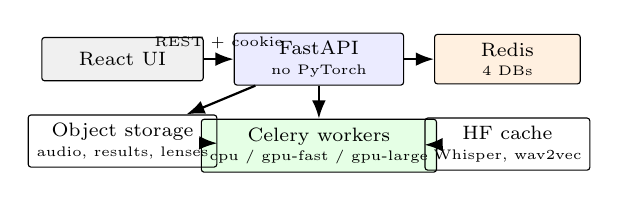
\begin{tikzpicture}[
  font=\scriptsize,
  box/.style={draw, rounded corners=1pt, align=center, inner sep=3pt, minimum height=0.55cm},
  arr/.style={-{Latex}, thick}
]
\node[box, fill=gray!12, minimum width=2.05cm] (ui) {React UI};
\node[box, fill=blue!8, minimum width=2.15cm, right=0.38cm of ui] (api) {FastAPI\\[-1pt]{\tiny no PyTorch}};
\node[box, fill=orange!12, minimum width=1.85cm, right=0.38cm of api] (redis) {Redis\\[-1pt]{\tiny 4 DBs}};
\node[box, fill=green!10, minimum width=2.15cm, below=0.42cm of api] (w) {Celery workers\\[-1pt]{\tiny cpu / gpu-fast / gpu-large}};
\node[box, minimum width=2.05cm, below=0.42cm of ui] (store) {Object storage\\[-1pt]{\tiny audio, results, lenses}};
\node[box, minimum width=1.85cm, below=0.42cm of redis] (hf) {HF cache\\[-1pt]{\tiny Whisper, wav2vec}};
\draw[arr] (ui) -- node[above, font=\tiny] {REST + cookie} (api);
\draw[arr] (api) -- (redis);
\draw[arr] (api) -- (w);
\draw[arr] (w) -- (store);
\draw[arr] (api) -- (store);
\draw[arr] (w) -- (hf);
\end{tikzpicture}
\caption{ECHO runtime. The API authorizes jobs and never loads weights. Workers own models, pull audio by opaque key, and write result artifacts. Redis holds sessions, job metadata, and the broker.}
\label{fig:arch}
\end{figure}

\subsection{Models and capabilities}

Three built-in models ship with a frozen capability set. Whisper-base and Whisper-large (\texttt{openai/whisper-large-v3}) are seq2seq ASR: prediction, embedding, attention, saliency, hidden states, layer probes, decoder activations, and Jacobian-lens fit/apply. The bundled wav2vec~2.0 checkpoint is audio classification (neutral, happy, sad, angry, fear): prediction, embedding, saliency, hidden states, and layer probes---no attention pairs, no decoder lens. A worker-side registry keys loaded weights by model, purpose, revision, and device so the eager-attention copy used for visualization is not the generation copy, and a saliency copy reserved for gradients is not evicted by an embedding pass.

Users may register a Hugging Face repository. Validation loads the model config and processor with remote code disabled, classifies the architecture as seq2seq ASR, CTC ASR, or audio classification, and assigns the matching capability set. CTC models have no decoder residual to unembed, so the Jacobian lens is withheld---the same gate as for wav2vec~2.0. Remote code is never executed during preflight.

\subsection{Datasets}

Built-in datasets are CSV-backed directories streamed with HTTP \texttt{Range} so the waveform can seek. Common Voice~\cite{ardila2020commonvoice} supplies read speech with optional age, gender, and accent columns. RAVDESS~\cite{livingstone2018ravdess} supplies acted emotion. LibriSpeech-1000~\cite{panayotov2015librispeech} is a 1000-clip read-speech slice used both as a browsing set and as a Jacobian-lens fit corpus. L2-ARCTIC~\cite{zhao2018l2arctic} adds non-native English with phone-level annotations used by fairness grounding. The Speech Accent Archive contributes accented read speech. Session-scoped custom datasets accept \texttt{.wav}, \texttt{.mp3}, \texttt{.m4a}, and \texttt{.flac} with optional transcript manifests; names are prefixed with the session identifier so they cannot collide across users.

\section{Interpretability Toolkit}

Each tool is a job (or an analysis chord) with a typed parameter schema. Extra fields are rejected. The UI is a shared layout: dataset table, waveform, prediction panel, and visualization tabs. Table~\ref{tab:questions} is the intended reading order, not a ranking of methods.

\begin{table}[!t]
\caption{Analyst questions and the ECHO tool that answers them.}
\label{tab:questions}
\centering
\setlength{\tabcolsep}{2.5pt}
\begin{tabular}{@{}p{0.46\columnwidth}p{0.46\columnwidth}@{}}
\toprule
Question & Tool \\
\midrule
What did the model emit? & prediction (WER/CER or class probs) \\
Where did the decoder look in the audio? & cross-attention pairs \\
Which waveform region moved the score? & saliency overlay \\
Which clips does the model treat as similar? & embeddings + HDBSCAN \\
How brittle is the prediction? & perturbations; FR-7 sweeps \\
At what encoder depth is property $X$ linear? & layer probes \\
Do groups differ in error or explanation quality? & FR-10 fairness + grounding \\
What is the decoder poised to say? & Jacobian lens \\
\bottomrule
\end{tabular}
\end{table}

\subsection{Prediction}

Whisper jobs return a transcript. When the row has a reference, the UI shows word and character error rates, Levenshtein distance, exact match, and character similarity, using Whisper's own English normalizer so numbers are comparable with published Whisper WER. wav2vec~2.0 jobs return a predicted emotion, a probability vector, and a confidence. Perturbing the clip re-runs the same job on the new asset so the analyst sees a paired before/after.

\subsection{Attention}

Whisper is loaded with \texttt{attn\_implementation="eager"}. Scaled-dot-product and FlashAttention paths silently drop attention tensors; without the eager flag the panel would be empty. The job returns, for a chosen layer and head, word-to-word weights merged with timestamped chunks into (word, time interval, weight) pairs and a timeline series. Cross-attention is the alignment question: which of the 1500 encoder frames a decoder position read. It is not a claim about what token the residual contains.

\subsection{Embeddings, projection, and clustering}

Each clip is mean-pooled from the encoder hidden state (512-D on Whisper-base). PCA, t-SNE, or UMAP~\cite{mcinnes2018umap} projects to 2-D or 3-D. Optional HDBSCAN~\cite{campello2013hdbscan} clusters the vectors, with a PCA pre-reduction above 50 dimensions because density clustering degrades in the native encoder width. The scatter plot supports click-to-select, box and lasso, and a 3-D plane picker. Dataset EDA---class balance, histograms, correlation, nearest neighbours---reads the same metadata and, when embeddings exist, the same coordinates. Clustering quality (silhouette, Davies--Bouldin, Calinski--Harabasz) is reported when the geometry supports it; degenerate sets return a well-formed empty payload rather than a partial schema.

\subsection{Saliency}

The job API exposes Grad-CAM~\cite{selvaraju2017gradcam}, LIME~\cite{ribeiro2016lime}, and KernelSHAP~\cite{lundberg2017shap}. The service also implements Integrated Gradients~\cite{sundararajan2017ig} and layer-wise relevance propagation. Scores are segment-level overlays on the waveform, optionally aligned to Whisper word chunks. Duration caps (12\,s default, 6\,s for SHAP) exist because SHAP scales poorly and long clips OOM the worker; an opt-in \texttt{full\_audio} flag bypasses the crop. Saliency answers a different question from attention: which input region moved a scalar, not where the decoder looked.

\subsection{Perturbations and linguistic-versus-acoustic sweeps}

Single-clip perturbations---Gaussian noise, time masking, pitch shift ($\pm 6$ semitones, $\le 30$\,s), time stretch---write a new audio asset and re-trigger prediction. FR-7 expands a grid of acoustic properties (noise, pitch, speed, time mask, frequency mask) plus an identity control and an optional lexical control, caps the grid at 60 variants, and estimates cost before submit. Each variant is re-inferred. ASR variants report WER against ground truth and against the identity transcript (self-WER); classification variants report confidence deltas and Jensen--Shannon divergence. The result is a sensitivity profile: which acoustic axis moves the model, and whether a linguistic control moves it more. This is behavioural testing in the spirit of CheckList~\cite{ribeiro2020checklist}, on audio axes rather than templates.

\subsection{Layer probes}

A probe job extracts mean-pooled encoder states at every recorded layer, including the embedding output, then trains a logistic regression or linear SVM per (property, layer) under stratified cross-validation. Labels come from dataset columns or a user-supplied map; empty, ``unknown'', and ``n/a'' are missing, not a class. Three numbers are always present~\cite{hewitt2019control,belinkov2022probing}: cross-validated accuracy, the majority-class baseline, and selectivity (accuracy minus a control probe trained on shuffled labels). Accuracy at or below majority means no information was found, however large the number looks. Accuracy above majority but not above the control is memorization of the split, not a readable representation. The UI plots a layer profile and a property-by-layer heatmap. Probes answer linear decodability of speaker, gender, emotion, or lexical tags; they are not maps onto the model's unembedding.

\subsection{Fairness and explanation grounding}

FR-10 takes a dataset and a grouping column (accent, gender, language, and other metadata that is not an identifier or free-text transcript). It classifies the design (whether groups share content, whether counts support a comparison), runs per-item inference, and aggregates WER or classification metrics with percentile bootstrap confidence intervals---not BCa, which would require a jackknife this module does not implement. Representational comparison uses embedding geometry (silhouette, nearest-neighbour group leakage).

Explanation fairness is a second pass. Existing saliency series are scored against an energy-based speech mask: grounding lift is the saliency mass on speech divided by the speech duty cycle, with entropy, Gini, and top-10 mass as companions. A group can have comparable WER and still have explanations that sit on silence. L2-ARCTIC phone annotations additionally support a phone-confusion view. Insufficient groups fail closed with a non-retryable error rather than a silent two-group plot.

\subsection{Decoder Jacobian lens}

For seq2seq ASR only, ECHO fits one Jacobian per decoder block,
$J_\ell=\mathbb{E}_{t,\,t'\ge t}[\partial h_{\mathrm{final},t'}/\partial h_{\ell,t}]$,
with Hutchinson probes~\cite{hutchinson1989trace}, and reads $\operatorname{softmax}(E J_\ell h_{\ell,t})$ through Whisper's tied projection~\cite{gurnee2026workspace}. The encoder runs under \texttt{no\_grad}. Current Hugging Face Whisper records six decoder-block states on the base model; a production fit on this codebase uses $N=1000$ transcripts and $P=4$ probes and writes six $512\times 512$ maps. Apply returns a $(\text{position}\times\text{layer})$ top-$k$ grid. Mid layers tend to reconstruct the current token and a semantic neighbourhood; the last layer tends toward the next token, start-of-transcript language identity, and end-of-text stop planning. Display softmax is not calibrated confidence. CTC and classification models are excluded because they have no decoder residual to unembed. The estimator, the encoder-transport failure, and the linear closed-form test (relative Frobenius error $<0.1$ on a stub decoder) are the subject of the companion short paper; this paper only records that the lens is a job on the same workbench as attention and saliency, answering a question those panels do not.

\section{Implementation Notes}

Several constraints are load-bearing.

\paragraph{Eager attention.}
Whisper attention jobs instantiate the model with \texttt{attn\_implementation="eager"}. The GPU eager path has additionally been observed to fault through Triton's batched-matmul kernel; an \texttt{ATTENTION\_FORCE\_CPU} pin exists for that case.

\paragraph{Control-plane imports.}
Planning helpers for FR-7 and FR-10 (cost estimates, groupable columns, design classification) use only the standard library so the API container can import them. Numpy, librosa, jiwer, and scikit-learn stay behind local imports in worker-only functions.

\paragraph{Cache identity.}
Results are keyed by operation, model revision, audio identity, and the parameter fields that change the computation. Hidden-state extraction and layer probes share per-file activation cache entries: changing probe hyperparameters retrains without re-running the encoder. Saliency keys embed a schema version (\texttt{v2}) so a response-shape change invalidates rather than migrates.

\paragraph{Session isolation.}
A session cookie (HTTP-only, SameSite lax) scopes custom datasets, custom models, and lens artifacts. Cross-session \texttt{get\_owned} returns nothing. That is a security boundary, not a convenience.

\paragraph{Queue and time limits.}
Soft/hard Celery limits are 55/60 minutes. Lens fit on 1000 clips is a \texttt{gpu-large} job; SHAP on a long clip is not. Prefork workers pin OpenMP/BLAS to one thread and force Numba onto a generic CPU target: native feature detection in this container produced SIGSEGV on first librosa JIT.

\paragraph{Tests.}
The suite covers job contracts, session ownership, cache policy, FR-7 DSP invariants and metrics, FR-10 API/orchestration/grounding, layer-probe schemas, the Jacobian closed form, and security. It does not substitute for a corpus-level interpretability evaluation.

\section{Using ECHO}

A typical session is a loop, not a single plot. Pick Whisper-base and Common Voice. Select a row; prediction fills WER against the reference. Open attention on a late layer: if the spoken word aligns to a silence pad, the failure is not (only) a language-model prior. Open saliency on the same clip: if Grad-CAM mass is off-speech, grounding lift will say so, and a fairness run grouped by accent will show whether that is group-systematic. Extract embeddings for the slice; lasso a cluster that is all one speaker. Probe gender and accent across encoder layers: a property that peaks early and collapses is a candidate for a surface cue; a property that peaks late is a candidate for a task feature. Perturb with noise and re-apply the Jacobian lens on the same reference transcript: a late-layer ranking that flips while mid layers still show the spoken word is a different diagnosis from a column that never ranked it.

None of these steps is an automatic detector. The workbench's job is to put the complementary views on one clip so the analyst can choose the next measurement---more audio, a different decoding setup, a group-level fairness run, or a probe at one depth instead of all of them.

\section{Limitations}

ECHO is not a user study; we do not report time-to-insight or preference against a script-only baseline. Saliency duration caps and SHAP's sample count are operational, not theoretically optimal. Layer probes are linear and pooled; they cannot speak to non-linear or frame-level phonetic structure. Fairness requires a groupable metadata column and enough items per group; many uploads will not qualify. The Jacobian lens is first-order, teacher-forced, revision-bound, and seq2seq-only; $P=4$ leaves probe noise. Custom models refuse \texttt{trust\_remote\_code}, which excludes some community checkpoints. There is no streaming path, no write/steer/ablate mode, and no third-party method plugin. Built-in datasets are subsets, not full releases.

\section{Conclusion}

ECHO is a LIT for speech: a control plane that never loads weights, workers that do, and a toolkit whose members are useful because they disagree. Attention locates an encoder frame; saliency locates a waveform region; probes locate a depth at which a property is linear; fairness locates a group; the Jacobian lens locates a verbal ranking in the decoder. Shipping them on one session does not make any one estimator faithful~\cite{jacovi2020faithfulness}. It does make the next question cheaper to ask. The measurements that would make the systems claim as strong as a methods claim---a workspace-band census, a fairness replication of known ASR disparities inside the UI, a small analyst study---should be taken on this workbench rather than on a fresh pile of scripts.

\section*{Acknowledgments}

We thank Dr.~Uthayasanker Thayasivam for guidance. The Jacobian-lens estimator follows Gurnee et~al.~\cite{gurnee2026workspace}; remaining errors are ours.

\balance
\bibliographystyle{IEEEtran}
\bibliography{references}

\end{document}
